\section{Hombre de Vitruvio} \label{app:vitruvio}

\begin{figure}[H]
    \centering
    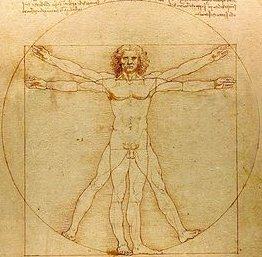
\includegraphics[width=0.35\textwidth]{vitruvio2.jpg}
    \caption{Hombre de Vitruvio, el dibujo más conocido de Leonardo Da Vinci} % URL:http://upload.wikimedia.org/wikipedia/commons/thumb/2/22/Da_Vinci_Vitruve_Luc_Viatour.jpg/300px-Da_Vinci_Vitruve_Luc_Viatour.jpg
\end{figure}

\section{Andrés Vesalio} \label{app:vesalio}

Andrés Vesalio fue un pionero en el ámbito de la anatomía. En su tratado ``De humani corporis fabrica" se pueden apreciar diversas representaciones de la anatomía del cuerpo humano en movimiento. A continuación están detallados algunos de estos dibujos:
\begin{figure}[H]
    \centering
        \begin{subfigure}[b]{0.28\textwidth}
             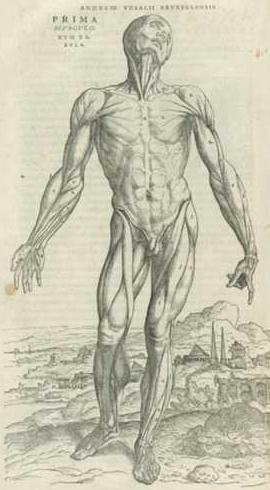
\includegraphics[height=6cm]{musculos.jpg}
             \caption{Músculos}
        \end{subfigure}
        \begin{subfigure}[b]{0.28\textwidth}
             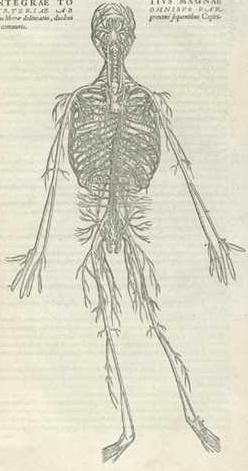
\includegraphics[height=6cm]{nervios.jpg}
             \caption{Nervios}
        \end{subfigure}
        \begin{subfigure}[b]{0.28\textwidth}
            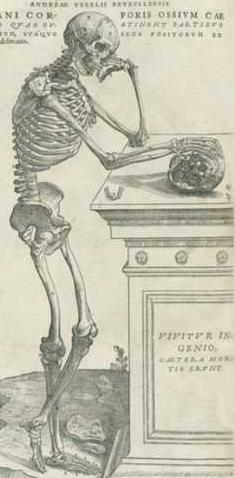
\includegraphics[height=6cm]{esqueleto.jpg}
            \caption{Esqueleto}
        \end{subfigure}
        \begin{subfigure}[b]{0.37\textwidth}
             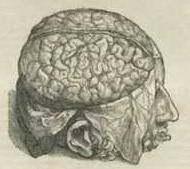
\includegraphics[width=\textwidth]{cabeza.jpg}
             \caption{Cabeza y cerebro}
        \end{subfigure}
        \begin{subfigure}[b]{0.3\textwidth}
             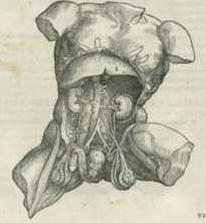
\includegraphics[width=\textwidth]{interior.jpg}
             \caption{Órganos internos}
        \end{subfigure}
\end{figure}
% http://www.biografiasyvidas.com/biografia/v/vesalio.htm
% http://archive.nlm.nih.gov/proj/ttp/flash/vesalius/vesalius.html
% http://quod.lib.umich.edu/w/wantz/vesd1.htm
% Andrés Vesalio, su vida y su obra Escrito por José Barón Fernández